% Summary if this section

The first step of the development process, defined in Section~\ref{subsec:dev_process}, consists of identifying what the delta-rs library (version 0.15.x) lacks to satisfy the requirements, more specifically, how to support \gls{HDFS} and \gls{HopsFS} in the delta-rs library. This step outlines the library structure (colloquially defined as "crate") divided into sublibraries (colloquially defined as "subcrates"), which is illustrated in Figure~\ref{fig:delta-rs_schema}. As the figure shows, the delta-rs crate has a subcrate for each storage connector, so adding support for different storage is a matter of implementing a new subcrate to the delta-rs crate.

\begin{figure}[!ht]
    \begin{center}
      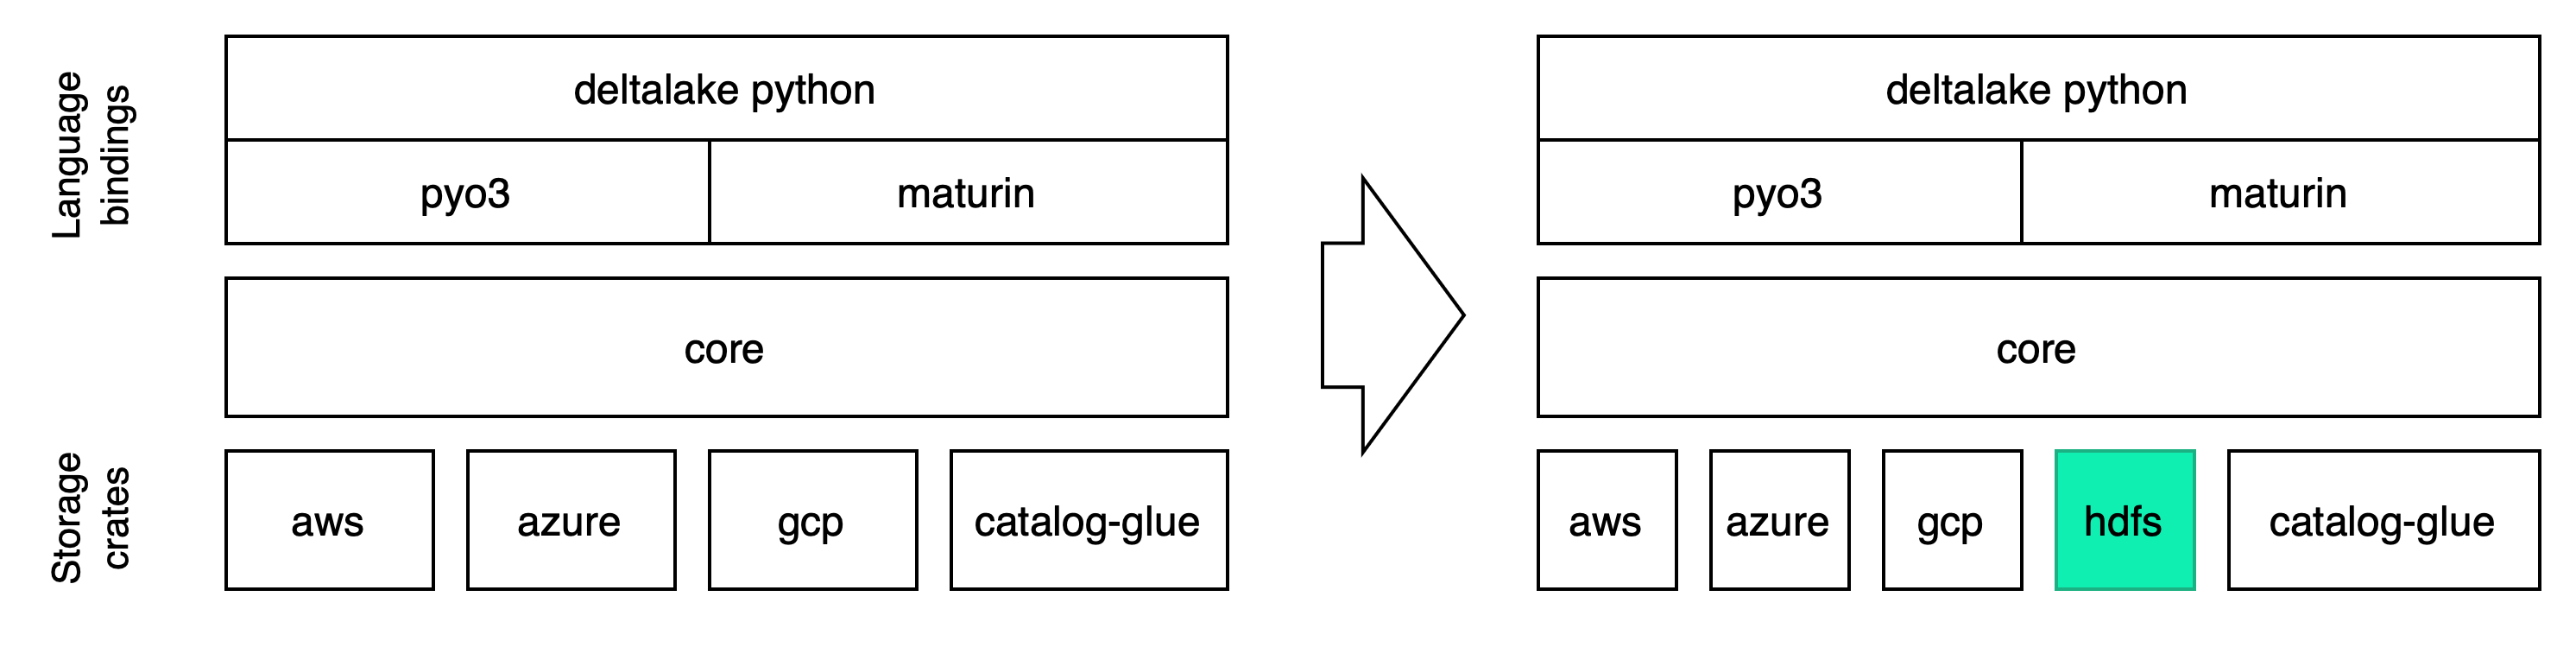
\includegraphics[width=\textwidth]{figures/4-implementation/delta-rs_schema.png}
    \caption[Delta-rs architecture before and after implementation]{Delta-rs library (v. 0.15.x) before and after adding \glstext{HDFS} support. Diagram inspired by delta-rs architecture presented by R. Tyler Croy at the Data+AI Summit 2021. Recording available at \url{https://www.youtube.com/watch?v=scYz12UK-OY&t=585s}.}
    \label{fig:delta-rs_schema}
    \end{center}
\end{figure}

The delta-rs library uses an external interface called object-store defined in the Arrow-rs library~\footnote{Project's repository available at \url{https://github.com/apache/arrow-rs/tree/master/object_store}}. Every storage connector implements this interface, and the other parts of the library interact with the storage layer. Thus, the new \gls{HDFS} storage must also implement this interface.

The development process was divided into two subsections: a first approach and a final approach. The first approach was carried out by developing a \gls{HDFS} subcrate for the delta-rs crate from scratch, while the second and final approach modified the support for \gls{HDFS} added in delta-rs with version 0.18.2 to also support \gls{HopsFS}. These approaches follow the major development iterations of this project, which also consider the contributions to the delta-rs library.

\subsection{First approach}
% Describe the first approach trying to implement object_store for HDFS
At the beginning of the project, a first approach was taken to provide support for \gls{HDFS} to the delta-rs library version 0.15.x. Analyzing past contributions to the library reveals that \gls{HDFS} was supported in version 0.9.0 of the delta-rs library, but support was removed due to three main reasons:
\begin{enumerate}
  \item The \gls{HDFS} support caused the testing pipeline to fail, and no trivial solution was found.
  \item The \gls{HDFS} support had \gls{JVM} dependencies. This was considered a strong limitation for Python users, as having Java installed is high overhead (in terms of storage and computation) for performing an operation in Python. Having these Java dependencies would have meant that many Python users would not have used the library altogether.
  \item The community around the library did not have contributors or many users, which had \gls{HDFS} as a use case.
\end{enumerate}
Starting from the \gls{HDFS} support in the delta-rs library in version 0.9.0, a solution was designed to fix the testing issues and provide a working storage support for \gls{HDFS}. The architecture is described in Figure \ref{fig:approach_1_solution_schema}. 

\begin{figure}[!ht]
  \begin{center}
    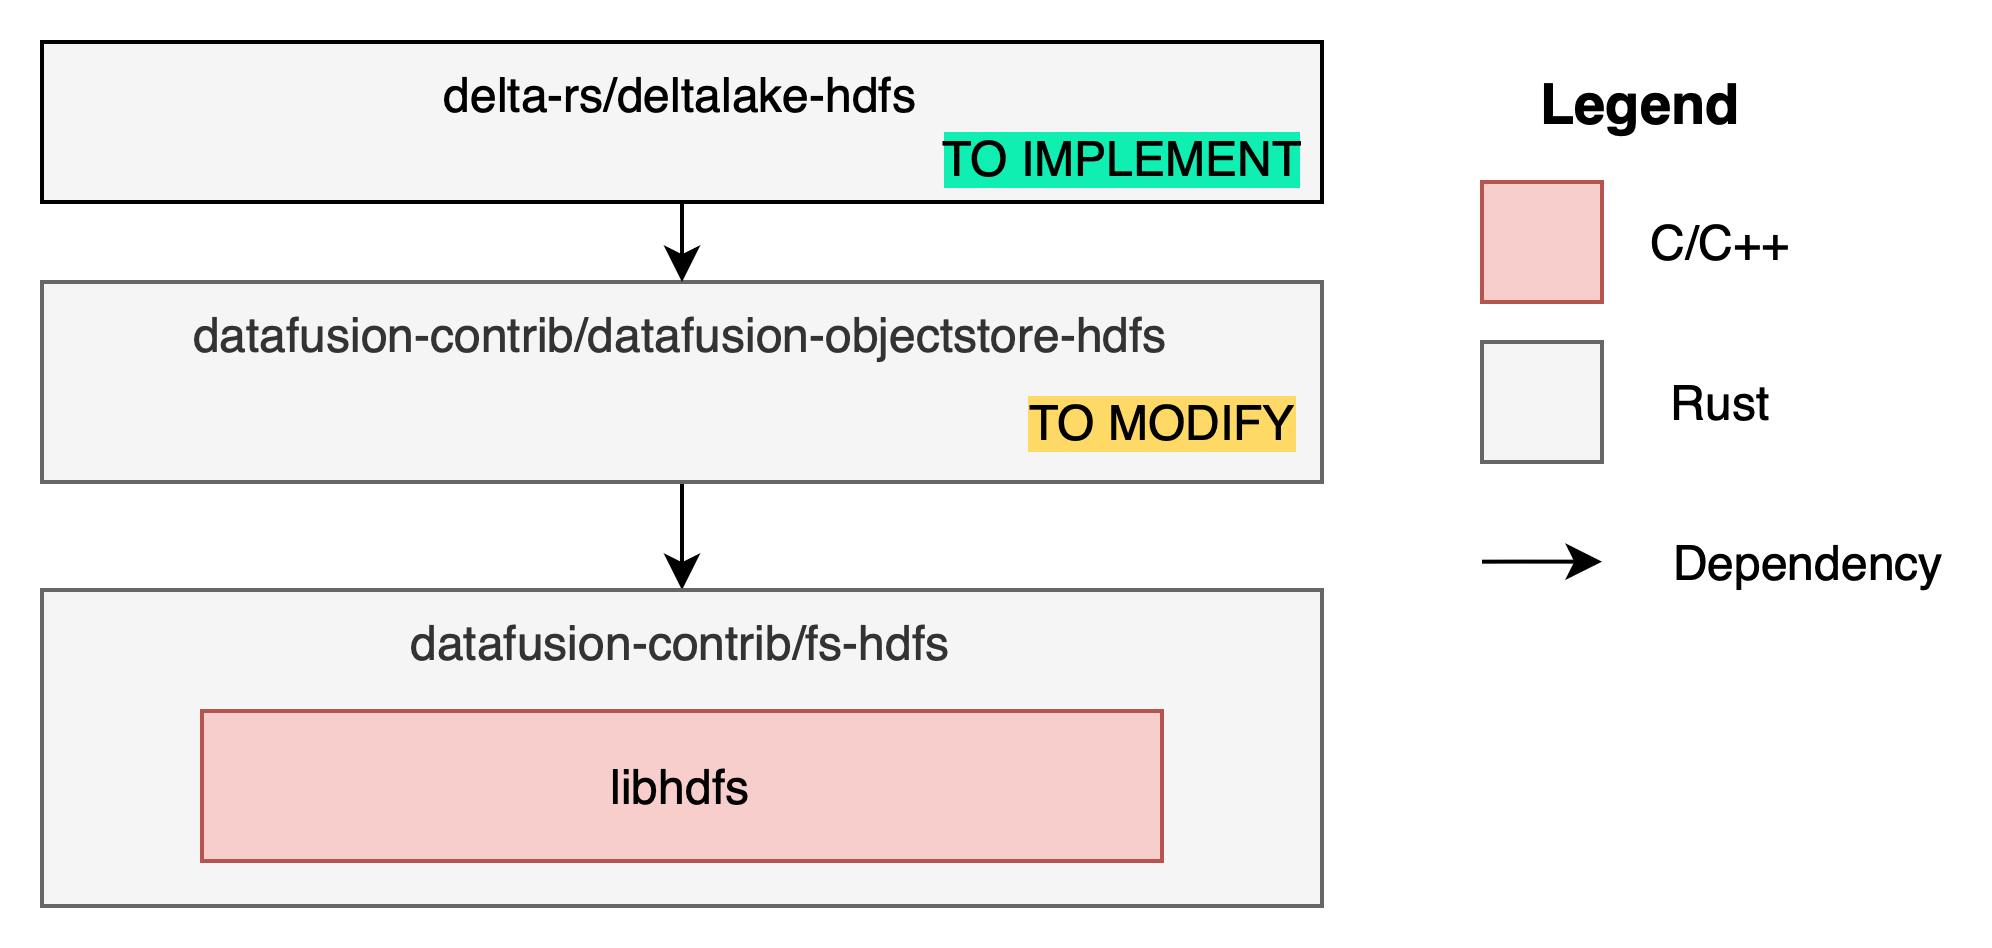
\includegraphics[width=\textwidth]{figures/4-implementation/approach1_solution_schema.png}
  \caption[First solution architecture]{Architecture of the first implementation approach. The repositories that need to be implemented or modified are highlighted in green and yellow, respectively.}
  \label{fig:approach_1_solution_schema}
  \end{center}
\end{figure}

This implementation uses a C++ library called libhdfs, which contains all the methods required to work as an \gls{HDFS} client. This library is contained in the Rust library fs-hdfs. The datafusion-objectstore-hdfs uses the libhdfs library to provide an interface for \gls{HDFS} that implements object-store, the interface used in the delta-rs library to interact with storage connectors.

This approach first required the rewrite of the datafusion-objectstore-hdfs as it used an older object-store interface version (0.8.0 vs. 0.10.0), and it was no longer possible to upgrade it easily. Secondly, the \gls{JVM} dependencies, while this project did not have a strict requirement on not having them, being able to have the dependencies consistently work on different development environments proved to be a challenge. 

Ultimately, this approach was abandoned following the release of version 0.18.2 of the delta-rs library. This decision was taken to comply with the maintainability requirement defined in Section \ref{subsec:requirements}.

\subsection{Final solution}
% Describe the second approach by modifying the HDFS-NATIVE library

Version 0.18.2 of the delta-rs introduced support for \gls{HDFS} via the hdfs-native library~\footnote{Project's repository available at \url{https://github.com/Kimahriman/hdfs-native}}. This is a Rust library that re-implements the \gls{HDFS} client, avoiding the use of libhdfs, and thus has no \gls{JVM} dependencies. This architecture is illustrated in Figure~\ref{fig:approach_2_solution_schema}.

\begin{figure}[!ht]
  \begin{center}
    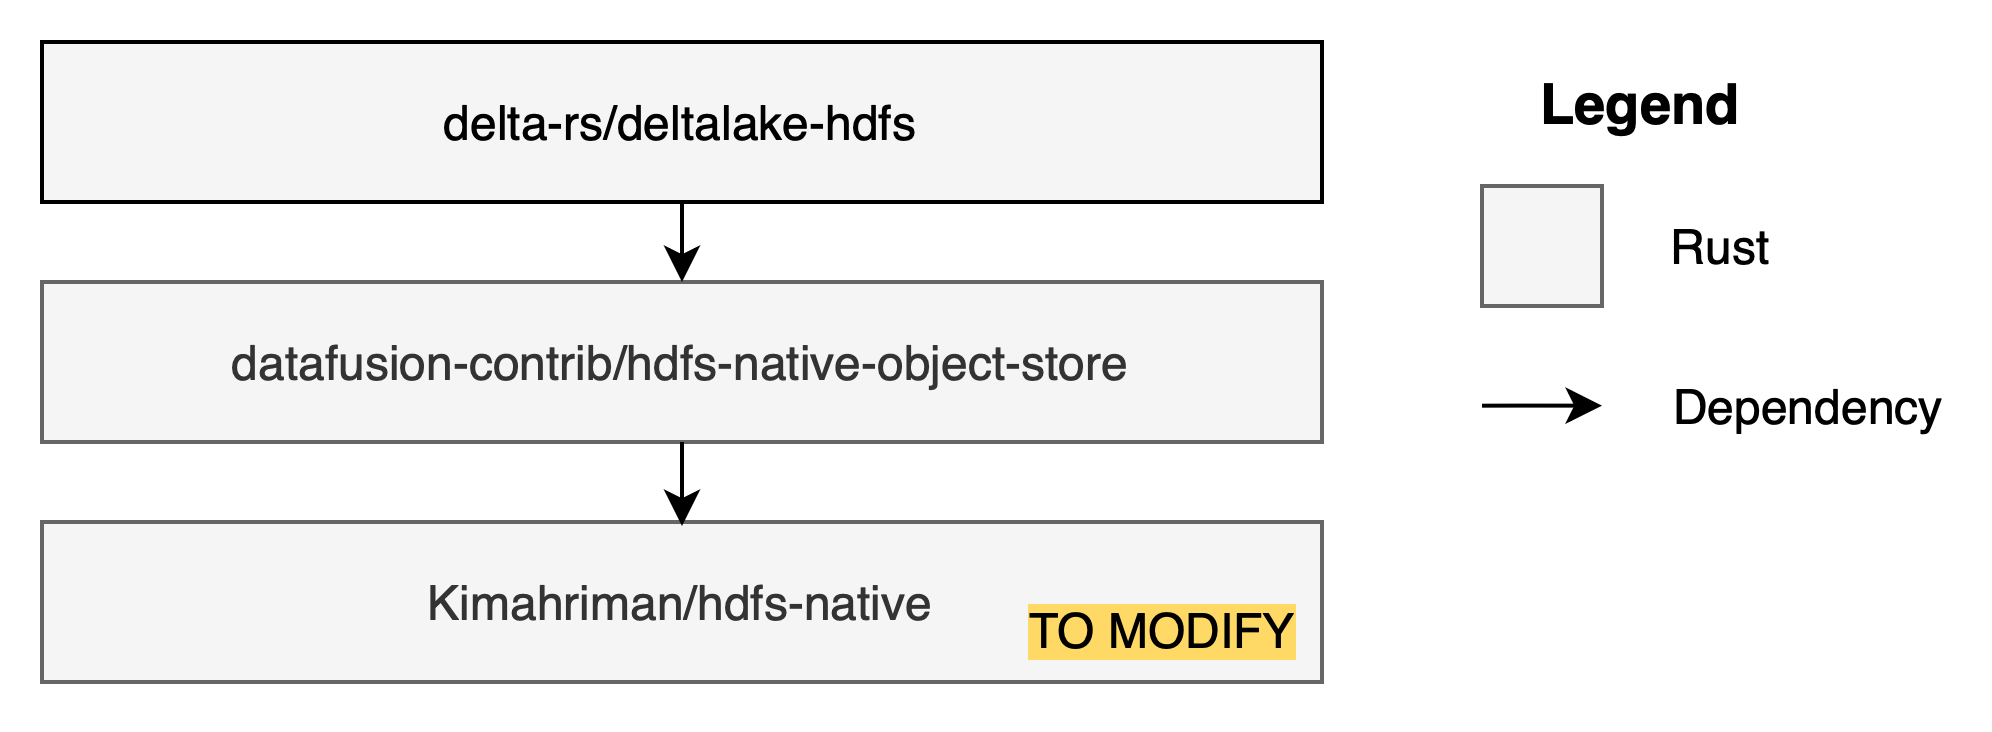
\includegraphics[width=\textwidth]{figures/4-implementation/hdfs-native.png}
  \caption[Final solution architecture]{Architecture of the final implementation approach. The repositories that need to be modified are highlighted in yellow.}
  \label{fig:approach_2_solution_schema}
  \end{center}
\end{figure}

While being used by the delta-rs library, this approach had some incompatibilities with \gls{HopsFS}. Here below is a list of them:
\begin{enumerate}
  \item \textbf{Different \glsentryshort{HDFS} protocol version}: \gls{HDFS} makes use of a \gls{RPC} protocol to interact with a \gls{HDFS} client. Hdfs-native is based on protocol version 3.2, while \gls{HopsFS} was compatible with version 2.7.
  \item \textbf{No support for \glsentryshort{TLS} in hdfs-native}: hdfs-native security is based on Kerberos, but it does not secure packet transfers using \gls{TLS}.
\end{enumerate}
These incompatibilities were solved one by one during development in the following way:
\begin{enumerate}
  \item \textbf{Upgrading \glsentryshort{HopsFS} protocol version}: together with the industrial supervisor responsible for the maintenance of \gls{HopsFS}, the differences between the two protocol versions (2.7 vs. 3.2) were highlighted, and one by one resolved. This way, version 3.2.0.14 of \gls{HopsFS} was released, adding support to the \gls{HDFS} \gls{RPC} protocol version 3.2, making \gls{HopsFS} compatible with the hdfs-native library.
  \item \textbf{Adding support for \glsentryshort{TLS} in the hdfs-native library}: \gls{TLS} support to hdfs-native was added via the use of an external Rust library called tokio-rustls version 0.26~\footnote{Library available at \url{https://github.com/rustls/tokio-rustls}}.
\end{enumerate}

All changes were applied to copies (colloquially known as "forks") of the open-source repositories related to this project, namely delta-rs~\footnote{Code available at \url{https://github.com/Silemo/delta-rs}}, hdfs-native-object-store~\footnote{Code available at \url{https://github.com/Silemo/hdfs-native-object-store}}, and hdfs-native~\footnote{Code available at \url{https://github.com/Silemo/hdfs-native}}.